\documentclass[10pt,a4paper]{book}

\usepackage[utf8]{inputenc}
\usepackage[english]{babel}
\usepackage[english]{isodate}
\usepackage[parfill]{parskip}
\usepackage{tikz}
\usetikzlibrary{decorations.pathreplacing,shapes,arrows,positioning}
\usetikzlibrary{positioning}

\tikzstyle{input} = [coordinate]
\tikzstyle{output} = [coordinate]
\tikzstyle{block} = [rectangle, draw, text width=5em, text centered,  minimum height=4em]
\tikzstyle{storage} = [cylinder, shape border rotate=90, aspect=0.25, draw]
\begin{document}
% \maketitle\tableofcontents\newpage
\pagenumbering{Roman}
\tableofcontents
\newpage
% \listoffigures
% \newpage
% \listoftables
% \newpage
\pagenumbering{arabic}

\chapter{Planing}
\section{Idea}
\section{System diagram}
\begin{figure}[h!]
% \centered
\small
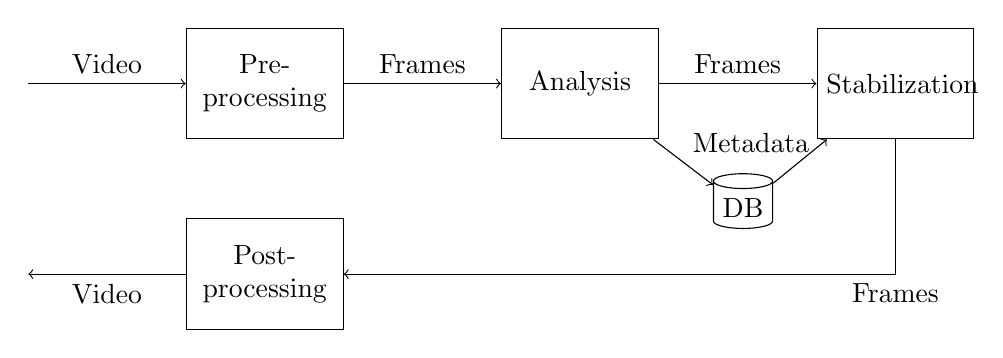
\begin{tikzpicture}[node distance=1cm and 2cm,auto]
    \node [input, name=input] {};
    \node [block, right= of input] (pre) {Pre-processing};
    \node [block, right= of pre] (analysis) {Analysis};
    \node [block, right= of analysis] (stabi) {Stabilization};
    \node [block, below= of pre] (post) {Post-processing};
    \node [input, left=of post] (output) {t};

    \node [storage, below right=0.5cm and 0.7cm of analysis] (analysisstorage) {DB};

     \draw[->](input) -- node {Video}(pre);
     \draw[->](pre) -- node {Frames}(analysis);
     \draw[->](analysis) -- node {Frames}(stabi);
     \draw[->](analysis) -- node {Metadata}(analysisstorage);
     \draw[->](analysisstorage) -- node {}(stabi);
     \draw[->](stabi) |- node {Frames}(post);
     \draw[->](post) -- node {Video}(output);
\end{tikzpicture}
\caption{High-level system diagram}
\end{figure}

%%%%%%%%%%%%%%%%%%%%%%%%%%%%%%%%%%%%%%%%%%%%%%%%%%%%%%%%%%%%%%%%%%%%%%%%%%%%%%%%
%%%%%%%%%%%%%%%%%%%%%%%%%%%%%% LOWER LEVEL SD %%%%%%%%%%%%%%%%%%%%%%%%%%%%%%%%%%
%%%%%%%%%%%%%%%%%%%%%%%%%%%%%%%%%%%%%%%%%%%%%%%%%%%%%%%%%%%%%%%%%%%%%%%%%%%%%%%%

\begin{figure}[h!]
% \centered
\small
\begin{tikzpicture}[node distance=1cm and 2cm,auto]
    \node [input, name=input] {};
    \node [block, right= of input] (first) {Pre-processing};
    \node [block, below= of first] (last) {Pre-processing};
    \node [input, left=of last] (output) {t};

    % \node [storage, below right=0.5cm and 0.7cm of analysis] (analysisstorage) {DB};

     \draw[->](input) -- node {Video}(first);
     \draw[->](first) -- node {Frames}(analysis);

     \draw[->](last) -- node {Frames}(output);
\end{tikzpicture}
\caption{Detailed system diagram of the \textit{Preprocessing}}
\end{figure}



\end{document}
